\documentclass[a5paper]{scrartcl}
%\documentclass[emulatestandardclasses, a5paper]{scrartcl}
\usepackage[margin=7mm]{geometry}
\usepackage{graphicx}
\usepackage{color}
\usepackage[ngerman]{babel}
\usepackage{hyperref}
%\usepackage{fullpage}
\usepackage{calc} 
\usepackage{enumitem}
\usepackage{titlesec}
\newcommand{\todo}[1]{\textcolor{red}{TODO: #1}\PackageWarning{TODO:}{#1!}}
\date{\vspace{-3ex}}
\begin{document}

\title{
	\includegraphics*[width=0.75\textwidth]{images/hu_logo.png}\\
	\vspace{24pt}
	Einf"uhrung in die \\ Architektur der Moderne\\ Konzeptionen, Imaginationen,\\ mediale Rezeption}
\subtitle{Proseminar WS 16/17\\
          Prof. Dr. Kai Kappel\\
          Institut f"ur Kunst- und Bildgeschichte \\ 
          Humboldt Universit"at zu Berlin}
\author{Lennard Wolf\\
        \small{\href{mailto:lennard.wolf@student.hu-berlin.de}{lennard.wolf@student.hu-berlin.de}}}
\maketitle
\begin{abstract}

Das einf"uhrende Seminar er"offnet kritische Zug"ange zur Begriffsbildung, Theorie und den wichtigsten Str"omungen der modernen Architektur. 

\end{abstract}
\newpage

\tableofcontents

%\listoffigures
\newpage


\section{Einf"uhrende Sitzung\\(18.10.16)}
\subsection{Organisatorisches}

\subsubsection{Grunds"atzliches}

\begin{itemize}
    \item Erste beide Semester sind Grundlagenmodule und zu belegen
    \item Klausur wird geschrieben, erste und einzige in 1. Sem
    \item Struktur: "Uberblicksvorlesung + Proseminar + Tutorium
    \item MAP: Referat mit Team (ganzer Monat; MAP wird bei Agnes angemeldet)
    \item Moodle pw: \emph{Stahltr"ager}
    \item Pflichtsprechstunde vor dem Vortrag
\end{itemize}

\subsubsection{Vortrag}

\begin{itemize}
    \item \emph{Le Corbusiers Konzept einer Ville Contemporaine}; 20min, 1 Handout A4
    \item Aufgabe dabei: Sagen, was die Bauten verk"orpern, die Ideengeschichte dahinter. Ob erst geb"aude und dann idee oder andersherum h"angt vom Vortrag ab
    \item Auch Kritik an m"oglichen Erkl"arungen aus Geschichtsb"uchern "uben (wenn angebracht)
    \item Mindestens 5 -- 10 Quellenangaben auf dem Handout. Auch bei Kubikat und Art historica (?) schauen! Nicht nur Primus B"ucher nennen. Handout bei Moodle hochladen, \emph{am besten eine Woche vorher}! 
    \item Folien immer als \texttt{.ppt}! Mit extrem hochaufl"osenden Bildern.
    \item Diskussionsfrage parat haben!
    \item Beim Vortrag stehen!
    \item Charakterisierung von Stil stark argumentativ begr"unden
    \item Die Zeit | Das Leben | Das Werk
\end{itemize}



\subsubsection{Klausur}
Handouts der Vortr"age sind Lernquellen.
Benotet??

\subsection{Einf"uhrung}
\subsubsection{Definitionen der Moderne?}
\begin{itemize}
    \item Haeufig sagt man: nach dem ersten Weltkrieg 1918 (Bauhaus)
    \item Aber: Jugendstil, Reformarchitektur, Eisen \& Stahlkonstruktionen etc..?
    \item Baustoffe, Schmuck etc.
    \item Seminar setzt im 19.Jh. an
\end{itemize}

\subsubsection{Wann endet die Moderne?}

\begin{itemize}
    \item Postmoderne, Zweite Moderne etc.?
    \item \emph{Modern is not contemporary}
\end{itemize}

\section{Wie beschreibe und analysiere ich moderne Architektur?\\(25.10.16)}

Treffen an der Ged"achtniskirche


\section{Zum Modernebegriff (nicht nur) in der Architektur\\(01.11.16)}

\subsection{Vornotizen}
\textbf{Definitionen und Abgrenzungen von Moderne}

\begin{description}[leftmargin=!,labelwidth=\widthof{\bfseries P2}]
  \item[Greenberg (Arch.)] \emph{Moderne Architektur bedeutet -- vereinacht gesagt -- funktionelle, geometrische Strenge und das Vermeiden von Dekoration und Ornament.} | Kap. `Modern und postmodern', Die Essenz der Moderne 
  \item[Greenberg (Kunst)] Bezeichnet K"unstler der Moderne als \emph{unbeugsamen Helden, der sich auf keinerlei Kompromisse mit dem Bestehenden einl"a\ss t und allen Verlockungen der eleganten Welt edelm"utig widersteht}; \emph{Bedeutende Werke wird ein K"unstler nur zu Wege bringen, wenn er alle au\ss erk"unstlcihen Anspr"uche und Erwartungen abweist, um seine Arbeit ganz aus sich sekbst heraus zu begr"unden.} $\rightarrow$ Das Publikum wurde dem Autor nach immer verst"andnisloser. | \emph{..selbstkritische Besinnung der Kunst auf ihre ureigenen und spezifischen M"oglichkeiten ist, Greenberg zufolge, das Charakterisikum des `Modernismus' }
  
  \item[Kretschmer] Latein: \emph{der Gegenwart angeh"orig} | im 19.Jh. als Gegensatz zu \emph{vergangen} | `Siegeszug' erst nach WWII | \emph{Die Moderne ist generell eine von technischem Positivismus gekennzeichnete Emanzipationsbewegung zur Befreiung aus der Fremdbestimmung.} | \emph{Es ging um eine m"oglichst gute Versorgung der neuen Massengesellschaft.} 
\end{description}

\textbf{Besprechung der Notizen}

\begin{itemize}
  \item Probleme zum einen der Datierung und der begrifflichen Festsetzung
  \item Es ist schwer w"ahrend einer Zeit "uber diese Zeit selber zu reden
  \item Freigang: Es gibt keine gro\ss e Erz"ahlung! Es besteht aus vielerlei Nebenwegen.
  \item Es ist kein Stil, kein formaler Rahmen, keine feste Zeit
\end{itemize}


\subsection{Sitzungsvortrag}

\begin{itemize}
  \item Seit Sp"atantike (5.Jh.): Die noch selbst erlebt Zeit
  \item Neuzeit: Kunst/Architektur die nicht dezidiert von der antiken Bautradition ableitbar ist (Schon Hauch von Avantgarde)
  \item Moderne in Geisteswissenschaften: industrielle Revolution, AUfkl"arung und S"akularisierung | Moderne in Philosophie: Aufkl"arung
  \item Beginn zwischen sp"aten 18. und mittleren 19. Jh. $\rightarrow$ Zeit des "Ubergangs von einem feudalistischen zu einem b"urgerlichen Gesellschaftsmodell
  \item Erste Erw"ahung 1886 von Eugen Wolff im Kontext der Literatur
  \item Moderne ist kein Stil- oder Epochenbegriff, sondern die Bezeichnung einer intellektuell wie formal (materiell wie gestalterisch) au\ss erordentlich vielf"altigen Str"omung.
  \item Bedingt durch die z.T. neuen, z.T. nun industriell herstellbaren Materialien Eisen/Stahl, Glas und sp"ater Beton: Industiebauten, Verkehrsbauten, Messebauten des 19. und 20. Jh.s (Paxton, Fr\`{e}res, Eiffel: \emph{Historische Moderne}) 
  \item Hochhausbauten des sp"aten 19. und erszen Drittel des 20. Jh.s in den USA; Arts and Crafts Architektur; Reformarchitektur (Jugendstil bzw. Wiener Sezession, Gartenstadtbewegung, Deutscher Werkbund, Darmst"adter Mathildenh"ohe, heimatbezofene Architektur)
  \item Klassiche Moderne 1910-1933 (Avantgardistische Architektur, Expressionistische, Organische Architektur, Traditionalismus) und viele mehr...
  \item Metabolismus, Cities:Moving
\end{itemize}


\section{Stahl und Glaskonstruktionen: Weltausstellungen des 19. Jahrhunderts\\(15.11.16)}

\subsection{Vortrag: Crystal Palace}

\begin{itemize}
  \item Crystal Palace. Jospeh Pacton 1851 Weltausstellungen London Hyde Park
  \item Warum ist er Modern und warum ist er Schl"usselwerk?
  \item These: 
\end{itemize}

\subsubsection{Hintergrund}

\begin{itemize}
  \item Nationalismus etc.
  \item Weltausstellungen Ziele: Plattform Vergleich von G"utern, Absatz f"ordern, Nation vereinen, statt gewalt in Industrie konkurrieren
  \item Schnell, Bau sollte demontierbar sein und B"aume sollten
  \item keiner der eingereichten Bau wird angenommen, paxton nach 5 Monaten mit Fox anderson \& co fertig gestellt
  \item wurde sp"ater nochmal aufgebaut; ist 1936 abgebrannt
  \item Vorl"aufer: Great Conservatory, 1941 von Paxton
  \item Bau ohne Ger"uste, Arbeiter verschraubten auf Leitern und dann hielt sich das Konstrukt von allein
\end{itemize}

\subsubsection{Beschreibung}

\begin{itemize}
  \item Flache D"acher (???) viele kleine Satteld"acher, Wasser kann gut ablaufen
  \item Besteht aus ganz vielen kleinen Modulen
  \item Ebenerdig, von B"aumen umringt
  \item Fassade besteht aus aneinandergereiten Glass...
  \item Grundriss: 563m lang 142m breit, 24m maximal h"ohe
  \item Querschiff war erst nicht geplant, doch 2 Ulmen mussten in den Bau inkludiert werden
  \item Haupteingang im S"uden
  \item Machinenraum im kleinen Glashaus
  \item Glasplatten waren gr"osser nicht herstellbar, und so musste sie die gesamte Formation des Baus nach deren Gr"osse ausrichten (\emph{kleinste Einheit})
  \item Komplett unverkleidet $\rightarrow$ Struktur des Baus ist gut erkennbar von innen wie von au"sen
\end{itemize}

\subsubsection{Wirkung und Wirken}
\begin{itemize}
  \item \emph{Wahrnehmungsschock}; \emph{Aufl"osen der Raumgrenzen durch das Fehlen von W"anden}; \emph{Desorientierung} durch Licht das durch das Glasdach str"omt; \emph{Zweifel an Sicherheit}; Nutzen gibt Orientierung, Menschen werden; Semper: Keine Masse und Dekoratives, keine Feierlichkeit $\rightarrow$ \textbf{keine Architektur} sondern nur Nutzbau
  \item Druch die L"ange von fast 600m hatte der Bau eine fast unendliche Wirkung 
  \item Heute: symbol f"ur technischen Fortschritt, Wegbereiter zur Moderne
  \item Industriell vorfabrizierte Einzelteile
  \item Nutz statt Representativbau
  \item Rechenprozess ist Grundlage, nicht k"unstlerische Idee
  \item War gut f"ur neue industrielle Bauten die flexibel sein mussten (z.B. Kaufh"auser, Markthallen)
  \item neue Licht- und Luftgestaltung
  \item `Wendepunkt f"ur Entwicklung der Baugeschichte' | etwas "ubertrieben, eher: Bauten mit der selben \emph{technisierten} und effizienzorientierten Haltung
  \item Komplett ohne steinernem St"utzbau (im Gegensatz zu anderen Bauten wie Bahnh"ofen in Paris und London)
\end{itemize}


\subsection{Vortrag: Der Eiffelturm}

\subsubsection{Hintergrund}

\begin{itemize}
  \item Grund: Weltausstellung 1889 in Paris
  \item Ziel: Beeindrucken der Besucher
  \item Handelsminister: Ideenwettbewerb
  \item Eiffel hatte schon l"anger einen solchen Bau zum Ziel der riesig gro"s ist
  \item Eiffel hatte Apartment oben auf der Spitze
  \item 300m hoch
  \item wurde sp"ater zu einem Rundfunkturm
  \item Skelettbau der Freiheitsstatue
  \item 
\end{itemize}


\subsubsection{Beschreibung}

\begin{itemize}
  \item Quadratische Grundfl"ache 125m
  \item Steilaufragende Pyramide
  \item 3 Etagen, unterste mit verziertem Torbogen
  \item Stahlbeton
  \item Puddelverfahren: Stahl aus Roheisen satt Holzkohle
  \item Wie h"alt er sich: das Material! wiegt insgesamt 7000 Tonnen
  \item Einfaches Muster wirkt durch starke Wiederholung komplex
\end{itemize}


\subsubsection{Wirkung und Wirken}

\begin{itemize}
  \item Filigran und monstr"os zugleich
  \item L"oste Turmbauwelle aus
  \item Kritiker: K"unstlerisches Verbrechen gegen die Baukunst; Giraffenk"afig; Sinnlos
  \item Architekten fanden es unfein dass pl"otzlich Ingenieure bauen
  \item Nur weil er noch einen Bogen und ein paar Ornamente rangeklatscht bekommen hat ist es gleich Baukunst? 
  \item Modern weil: In die H"ohe gebaut, Ingenieursdenken, 
\end{itemize}


\section{Stahl und Glaskonstruktionen: Hochhausbauten\\(22.11.16)}

\subsection{Vortrag: Louis Sullivan}

\subsubsection{Eckdaten}

\begin{itemize}
  \item Geb. Boston 1856 (Sohn Europ"aischer Immigranten) 
  \item studierte 1872 Architektur am MIT
  \item brach Studium ab um bei Architekten in NYC zu arbeiten (Furnice \& Harold ?)
  \item Zog dann nach Philadelphia
  \item 1881 Architekten-Partnerschaft mit Adler
  \item Gest. 1924 in Chicago
\end{itemize}

\subsubsection{Welche Inspirationen hatte Sullivan f"ur seine Bauwerke?}

\begin{itemize}
  \item Identifizierte sich mit dem l"andlichen Amerika
  \item M"ochte Technisierung mit dem L"andlichen sowie Traditionellem in Einklang bringen
  \item Wollte Anspr"uche des modernen Lebens erf"ullen
  \item Au"seres soll Inneres nach au"sen tragen
\end{itemize}

\subsubsection{Was sind die Charateristika seines Stils?}

\begin{itemize}
  \item 'Nat"urliche', organische Form (Klima und Umgebung in den Entwurf mit einbeziehen)
  \item Mochte Ornamente, g"aben 'Pers"onlichkeit'
  \item Modern an seinem Stil war das Verwenden von selbst gestalteteten pflanzlichen Ornamenten, die nicht auf Mustern aus der Antike aufbauen
  \item \emph{Form follows function} meinte: Ornamentik muss sich nach dem Konzept des Hochhauses richten
\end{itemize}




\subsection{Vortrag: Wainwright Building (St. Louis)}

\subsubsection{Hintergrund}

\begin{itemize}
  \item Grund: Flexible Amerikanische Gro"sraumb"uros
  \item Neu waren Absturzsichere Fahrst"uhle
  \item Neu auch der Gedanke dass Geb"aude nicht mehr Antike Strukturen folgen m"ussen
\end{itemize}


\subsubsection{Beschreibung}

\begin{itemize}
  \item Im Innern Stahl: billig, hoch, feuerfest
  \item Au"sen mit Stein 
  \item 3 Gliederung wie Sullivan es danach immer gemacht hat
\end{itemize}


\subsubsection{Wirkung und Wirken}

\begin{itemize}
  \item \emph{Neue Ornamentik} f"ur die neuen Bauformen (Siehe auch Guaranty (?) Building)
\end{itemize}

\subsection{Vortrag: Seagram Building (NYC)}


\begin{itemize}
  \item Damals teuerstes Hochhaus
  \item Mies van der Rohe \& Philip Johnson ( van der Rohe war nicht zugelassen)
  \item Modern wegen Skelettbau, Glas- und Betonfassade
  \item Platz vor dem Bau um ihn betrachtbar zu machen
\end{itemize}



\section{Buildings to live in, not to look at. Absagen an die Gliederungen des Historismus\\(06.12.16)}


\subsection{Vortrag: William Morris}

\begin{itemize}
  \item \emph{Kunst hat notwenidgigen Platz im menschl Leben: Regeln zum Leben, und Regeln f"ur dieses}
  \item Besitz und Bildungsb"urgetum: politische und kultureller Kern
  \item Adel und Bauern verloren an Bedeutung
  \item Reiche Familie; studierte Architektur in Oxford, sollte einst Religion studieren
  \item Kam in Kontakt mit den Pr"araffaeliten
  \item Pr"araffaeliten: "Ol auf feuchtem Putz, Themen: Mythen und Sagen; h"aufig viktorianische Sch"onheiten
  \item Wollte Maler werden, wurde Mitglied bei der Oxford Union
  \item Red House als Hochzeitsgeschenk an Jane B. (?): Geburtsort der Arts \& Crafts
  \item Gegenbewegung zur Konsumkultur: Qualitative Hochwertige Produkte die man nicht h"aufig wegschmei"sen muss
  \item Handarbeit!
  \item Gr"undete (heutigen) National Trust zum Erhalt alter Geb"aude
  \item \emph{Joy of nature}
\end{itemize}


\subsection{Vortrag: Red House}

\textbf{Houses to live in, not to look at}

\subsubsection{Hintergrund}

\begin{itemize}
  \item 1851 Crystal Palace: Alles ganz anders, Leute mochten neue Materialien und Bauart
  \item William Morris: \emph{Verkr"uppelung menschlicher Tugenden und Schaffenskraft}
  \item Arts \& Crafts: Wirklich Sch"ones ist immer der Natur entnommen | Beispiel: Pugin: Nur unverputzter roter Backstein (St. Maries Grande, 1838)
  \item Ornamentik hat bei industriellen Geb"auden nichts mehr mit dem Geb"aude selbst zu tun (?)
  \item Gesamtkunstwerkt aus der Arts \& Crafts Bewegung

\end{itemize}

Sch"onheit der Natur stammt aus der Sch"onheit der Mathematik

\subsubsection{Beschreibung}

\begin{itemize}
  \item asymmetrische Villa, freistehend
  \item Von Innen nach Au"sen gebaut funktionales Anbringen von Fenstern
  \item Wenig Ornamentik $\rightarrow$ Backsteine wurden durch Musterung selbst zur Ornamentik
\end{itemize}


\subsubsection{Wirken}

\begin{itemize}
  \item Morris als 'Maschinenhasser'
  \item Arts \& Crafts Gilden $\rightarrow$  ganzheitliche Schulungen
  \item $\rightarrow$ Deutscher Werkbund
  \item Kann als Gegenbewegung zur Industrialisierung gesehen werden
\end{itemize}

\subsection{Vortrag: Adolf Loos}

\begin{itemize}
  \item 10.12.1870 in Br"unn geboren
  \item gestorben 23.08.1933 Bei Wien
  \item Kritiker der Wiener Architektur (Historismus, Jugenstil)
  \item Hisotrismus ist verlogen, man rennt nur dem Alten hinterher, Ornamentik nutzlos
  \item H"auser haben Zweck zu erf"ullen, nicht unn"otig Arbeitszeit und Materialien zu verschwenden
  \item Ehrensoll von der tcheschichen Republik
  \item Baute haupts"achlich Villen
  \item Haus am Michaelerplatz (1911, Wien)
\end{itemize}


\subsection{Vortrag: Ornament und Verbrechen}

\begin{itemize}
  \item Vorgetragen 1910 in Wien, 1929 erst auf Deutsch ver"offentlicht
  \item Die modernen sich kleidenden Menschen sind Degenerierte Aristokraten
  \item Wir modernen Menschen haben die Ornamentik "uberwunden
  \item Sklaverei des Ornaments (Einfaches Volk ist leichter zu regieren)
  \item Industrie will Konsum, 
  \item Verpulvern ist un"asthetisch
  \item Qualit"at vor Quantit"at
\end{itemize}


\section{Der Beitrag der Niederlande zum Neuen Wohnen\\(03.01.17)}


\subsection{Vortrag: Amsterdamer Schule}

\begin{itemize}
  \item Gegenbewegung zu Impressionismus (geschwungene Formen etc) (?)
  \item Historischer Kontext: Wohnungsnot
  \item Expressionistischer Detailreichtum: Kunsthandwerk, Bildhauerei etc
\end{itemize}

\subsection{Vortrag: Gerrit Thomas Rietveld/De Stijl}

asketischer Stil, beeinflusst vom Purismus Le Corbusiers

\section{Visionen des Wohnens auf dem Weg zu einem “International Style”\\(10.01.17)}

\subsection{Vortrag: Le Corbusier}

\subsection{Vortrag: Werkbundsiedlung}

\begin{itemize}
  \item Wohnungsnot: Stuttgarter Wohnungsbauprogramme
  \item Menschenw"urdige Unterbringung der Massen: neue Wohnart
  \item Werkbund Ausstellung 1927 in ganz Stuttgart
  \item Stuttgart sollte internationaler Anziehungspunkt werden
  \item 12 K"unstler/Firmen (Interessenverband), nur "`Fortschrittliche"' Architekten (Neues Bauen, Organisches Bauen etc.), Peter Behrens , 
  \item Vereinigung von Kunst und Technik: Bewusstsein f"ur Qualit"at und Kultur
  \item Leiter: Mies van der Rohe
  \item Leitfrage: Wie wohnen?
  \item Neue Konzepte: Normierung, Typisierung
\end{itemize}



\section{Das Bauhaus und seine mediale Vermittlung\\(17.01.17)}

\subsection{Vortrag: Das Haus am Horn (1923)}

\begin{itemize}
  \item Hintergund: Krisensituation nach WWI; Fr"uhe Weimarer Schule, Ideen und Lehrplan sind schon formuliert (Einfl"usse: Kandinsky, Klee, Gropius; Mystisch Expressionistische Pr"agung)
  \item Vorgestellt bei Bauhaus Ausstellung in Weimar, 1923; heute UNESCO Welterbe
  \item 12x12m Grundfl"ache (Quadrat), errichtet in 4 Monaten, Einfamilienhaus, \emph{Musterhaus}
  \item Ziel: Sollte alle Ideen des Bauhaus zum wirtschaftlichen, funktionalistischen Bauen repr"asentieren; Industrialisierung des Bauens (Materialien); Bauhaus musste dem Staat beweisen, dass das Bauhaus keine Geldverschwendung ist, sondern dass "okonomisches Bauen funktioniert und zukunftstr"achtig ist
  \item 8 kleine niedrigere R"aume um ein gro"ses, h"oheres Wohnzimmer (mit Oberlicht, 36qm); Kinderzimmer neben Damenzimmer, Esszimmer neben K"uche etc.
  \item 2 Schichten vorgefertigte Betonplatten mit Isolierung dazwischen
  \item Erste Einbauk"uche der Welt, alles notwendige ist von einer Seite erreichbar
  \item Gesamtkunstwerk: Zusammenarbeit von allem m"ochlichen Handwerk (Tischler, Weber, etc.)
  \item Kritik zu der Zeit: "`undeutsch, geschmacklos"', da nicht traditionell genug
  \item noch sehr konservative Raumeinteilung (getrennte Herren und Damenzimmer, Damenzimmer an Kindern dran)
\end{itemize}

\subsection{Vortrag: Das Bauhaus Dessau}

\begin{itemize}
  \item Zielgerichtet in die Moderne: Antiakademische Ausbildung hin zum neuen Menschen (Normale K"unstler wurden arbeitslos weil sie nicht zeitgem"a"s ausgebildet wurden)
  \item Walther Gropius: Schuhleistenfabrik, Deutschland sollte \emph{n"utzlich und begehrenswert werden}; WWI: an der Front; Keine Massenherstellung denn dies t"otet das Individuum; "`Endziel jeder k"unstlerischen Arbeit ist der Bau."'
  \item Stufenmodell: Student wurde Lehrling, Geselle, Jungmeister, Meister
  \item Bauhaus heute Synonym f"ur moderne, praktische, schicke Architektur
  \item Am Anfang eher "`Hippiekommune"' als ernsthafte Akademie die es sp"ater war
  \item Klee, Kandinsky, Moholi Nagy waren Professoren 
  \item Bauhaus wurde von Th"uringen finanziert: war politische Institution
  \item "`Kunst und Technik bilden eine neue Einheit."'
  \item Einfl"usse: Suprematismus...
  \item Nach Rechtsruck in Deutschland wurden Gelder gek"urzt, doch durch Geld aus Amerika wurde das Bauhaus Gropius wieder in Dessau neuer"offnet (mit neuem Schulgeb"aude von Gropius (Einweihung Dez. 1926)) 
  \item Nicht mehr Repr"asentativbau sondern Funktionsbau (von innen nach au"sen); Nach innen gestzte Pfeiler, Davor Curtain Wall; Atelierabschnitt
  \item Dessau: Freiheitliches Lebensgef"uhl, Parties, avantgardistisch; Weimar: "armliche Studenten
\end{itemize}

\subsection{Vortrag: Lucia Moholy und die Fotografie vom Bauhaus}

\begin{itemize}
  \item 18.02.1894, Atheistische J"udin, tschechische Muttersprache, Studium ENglisch und Philosophie, wurde Lehrerin, besucht Barkenhof
  \item War Anlaufstelle am Bauhaus f"ur alles Fotografische, war Basis der Publizit"at
  \item Man erkennt ihre Objektfotografie an den Zerknitterten einfarbigen Hintergrundfl"achen
  \item Meisterh"auser manchmal durch B"aume fotografiert, da die geraden Linien der Geb"aude f"ur sich selbst sprechen
  \item Interieurs nur bei Meisterh"ausern, immer diagonal aufgenommen (fr"uher morgen)
  \item Kunstlos sachlicher Stil, "`Passive K"unstlerin"'; Sie empfand sich als rezeptiv, nicht kreativ schaffend; Kompositionelle Unbek"ummertheit
  \item Ohne Moholys Fotografien w"are kaum noch etwas vom Bauhaus "ubrig
  \item Sind fand die richtige Form f"ur das Einfangen der Bauhausprojekte
\end{itemize}


\section{Praxistest: Siedlungen f"ur den "`neuen Menschen"'\\(24.01.17)}

\subsection{Vortrag: Bruno Taut - Hufeisensiedlung}

\begin{itemize}
  \item Bruno Taut und Martin Wagner: Neues Bauen
  \item Sozialdemokratische Einstellung als roter Faden
  \item Hufeisensiedlung (Britz), Bau ab 1925
  \item Wohnungsf"uhrsorge
  \item Gro"sz"ugige Gr"unfl"achen, Kirschb"aume, Hufeisenteich, Ziel auch: Intensiv benutzte Gartenfl"achen mit Eigenanbau von Nahrungsmitteln
  \item Akribische Fassadengestaltung: Ziegelsteine, Farbanstriche
  \item Gegen"uber: Krugpfuhlsiedlung
  \item 7 Bauabschnitte, 6 davon UNESCO Weltkurlturerbe
  \item Hufeisen als Symbol f"ur den "`Solidarischer Geimnschaftsgedanken"'
  \item 4 Normierte Wohnugstypen, 49, 62, qm
  \item Wohnung ist mehr als Schlafort: Erholungsst"atte f"ur alle Mitglieder der Familie
  \item "`Die neue Wohnung"', Wohnund zu \emph{tauten}: Komfortabel und Praktisch einrichten
  \item \emph{Anger}: bezeichnet ein meist grasbewachsenes Land oder einen Dorfplatz in Gemeinbesitz, der von allen Bewohnern der Stadt oder des Dorfes genutzt werden konnte.  Ort f"ur Feste (z. B. Osterfeuer), f"ur gemeinschaftliche Aktivit"aten (Dorfbackofen, gemeinschaftliches Schlachten) und konnte auch einen heiligen Kultplatz, Ort f"ur Ratsversammlungen (Thing) oder als Richtplatz f"ur das germanische Stammesrecht dienen. 
\end{itemize}


\subsection{Vortrag: Siedlung Dessau-T"orten}

\begin{itemize}
  \item split-level!
\end{itemize}


\begin{itemize}
  \item Siedlung: Ort an dem sich Menschen zum Gemeinsamen Leben zusammengefunden haben; Sesshafte Lebensform
  \item "`Erforsche Deinen Z"ogling"' (Rousseau); Der neue Mensch
  \item Der Mangel an preiswertem Wohnraum, der durch die Stagnation der Baut"atigkeit w"ahrend des Ersten Weltkriegs noch forciert wurde, f"uhrte seit Beginn der Weimarer Republik zu verst"arkten "offentlichen Anstrengungen im bis dahin weitgehend privaten Wohnungsbau. Unter der Pr"amisse Licht, Luft und Sonne sollten Wohnungen entstehen, die f"ur eine gro"se Bev"olkerungsschicht erschwinglich waren.
  \item Licht, Luft und Sonne; Reihenhaussiedlung, Nutzg"arten, Eigentum
  \item Auftraggeber: Stadt Dessau an Walther Gropius
  \item Wie konnte etwas mit dem traditionellen Bauen konkurrieren in Komfort und Preis?
  \item Die von 1926 bis 1928 im Auftrag der Stadt Dessau gebaute Siedlung T"orten entstand im Rahmen des Reichsheimst"attengesetzes, d. h., die H"auser waren von Anfang an im Besitz der Bewohner. Mit der „halbl"andlichen“ Siedlung wollte das Bauhaus Probleme des preisg"unstigen Massenwohnungsbaus praktisch l"osen.
  \item Gropius entwarf eine Reihenhaussiedlung mit Nutzg"arten von jeweils 350 bis 400 qm f"ur den Gem"useanbau und die Kleintierhaltung zur Selbstversorgung. In insgesamt drei Bauabschnitten entstanden 314 Reihenh"auser, die je nach Haustyp zwischen 57 und 75 qm Wohnfl"ache aufweisen. Die Haustypen wurden in verschiedenen Varianten gebaut, um in einem ab 1927 angelegten umfangreichen Versuchsprogramm der Reichsforschungsgesellschaft f"ur Wirtschaftlichkeit im Bau- und Wohnungswesen Aufschl"usse "uber eine rationelle Herstellung von Wohnbauten, aber auch "uber die Eignung neuer Baustoffe und Industrieprodukte zu erhalten. Die Baustelle war, einer Taktstraße "ahnlich, so organisiert, dass von spezialisierten Arbeitsbrigaden immer mehrere H"auser eines Bauabschnitts zugleich gebaut werden konnten. Die vor Ort vorgefertigten Bauteile wie z. B. sogenannte Rapidbalken aus Beton wurden mit einer kleinen Bahn transportiert und von Kr"anen bewegt.
  \item Die hellen Kuben sind spiegelbildlich zu Doppelh"ausern und zu Gruppen von vier bis zw"olf Einheiten zusammengefasst. Die Fassaden wurden durch vertikale und horizontale Fensterb"ander gegliedert; das Innere war in hellen Farben gehalten. F"ur die Inneneinrichtung boten die Bauhauswerkst"atten spezielle M"obel an, die jedoch keine K"aufer fanden. Die Konstruktion der H"auser ergab sich aus der Notwendigkeit kostensparenden Bauens: Die tragenden W"ande sind aus vorgefertigten, preiswerten Schlackenbetonhohlk"orpern errichtet, die Decken wurden aus armierten Stahlbetontr"agern hergestellt.
  \item Kurz nach Fertigstellung zeigten sich Bau- und Planungsm"angel, sodass die Eigent"umer und Bewohner schon bald zahlreiche Umbauten vornahmen. Die ersten Ver"anderungen vor allem der zu hoch gelegenen Fensterb"ander begannen zun"achst nach einem einheitlichen Plan im Jahr 1934. Von der urspr"unglichen Einheitlichkeit der Siedlung ist heute deshalb nur noch wenig zu sp"uren. Das Haus am Mittelring 38 wurde ab 1992 als erstes originalgetreu wiederhergestellt. Es wird heute von der Moses-Mendelssohn-Gesellschaft genutzt und ist ebenso zu besichtigen wie das Haus Kleinring 5. Seit 1994 existiert eine Erhaltungs- und Gestaltungssatzung zum Schutz des Orts- und Stra"senbilds in der Siedlung, mit der die baulichen Ma"snahmen mit der historischen Substanz in Einklang gebracht werden sollen.
  \item Henry Ford, Frederick Taylor: Vorbilder f"ur die "Okonomisierung des Bauens
\end{itemize}


\section{Nachkriegsarchitektur in West und Ost\\(31.01.17)}

\subsection{Intro Kappel}

\begin{itemize}
  \item Bisheriger Standpunkt: Wettschreit der Systeme - Ost West; Heute: Relativiert
  \item 1950-51: Tr"ummerzeit, 53: BRD Wirtschaftswunder
\end{itemize}


\subsection{Vortrag: Richard Neutra}

\begin{itemize}
  \item Geboren 1892 in Wien, T"atig in Kalifornien, Gestorben 1970 in Wuppertal (Herzversagen)
  \item Gelernt unter Adolf Loos: Ablehnung der Ornamente; 
  \item Vorbild: Frank Lloyd Wright - Organische Prinzipien: Harmonie mit Natur
  \item 1924 Chicago, 1925 Los Angeles
  \item Ausstellung "`Modern Architecture"' in New York mit Wright, van der Rohe, Le Corbusier
  \item Ber"uhmtestes Haus: Lovell Haus
  \item "`Neuer Kalifornischer Stil"': Platzierung der Geb"aude einfach in ihre Umgebung, \emph{Biorealismus}
  \item Bekanntes Muster: Spiderlegs (D"unne S"aulen); Flache D"acher; Curtain Walls
  \item Geb"aude ist Spiegel der Naturumgebung, Ort der Erholung
  \item Grenzt sich von Funktionalismus ab (Sullivan: Form follows function)
  \item Poolhaus: "`Desert House"'
\end{itemize}


\subsection{Vortrag: Le Corbusier: Unite D'Habitation}

\begin{itemize}
  \item Charta von Athen (1933): Arbeitsraum der Zukunft - Gro"ser Einfluss auf die moderne Architektur; Kredo: Licht, Luft und Sonne
  \item Problem: Soziale Trennung (s. Marseille)
  \item Serienproduktion (Wohneinheit), hoher Komfort, vertikale Stadt, L"osung der Wohnungsnot
  \item u.A. in Marseille und Berlin
  \item Strahlende Siedlung (Cite Radieuse): 18 Geschosse, 337 Maisonettes (1600 Menschen), Gesch"afte, Hotel, W"ascherei, Sporthalle, Kindergarten
  \item Stahlbeton, Farbigkeit T"uren, W"anden
  \item Zug"ange reduzieren indem Flur nur alle 3 Geschosse ist
\end{itemize}

\subsection{Vortrag: Stalinallee - Karl-Marx-Allee (Scharun?) - Bauphase I}

\begin{itemize}
  \item Friedrichshain: Stalinallee ist heute Karl-Marx-Allee und Frankfurter Allee
  \item Radialstra"se (wie auch Prenzlauer Allee)
  \item 6.6km, 90m breit, "`letzter gro"ser europ"aische Boulevard"'
  \item Architektonische \emph{Auflockerung} der Stadt nach WWII $\rightarrow$ neue M"oglichkeiten der Stadtplanung
  \item Generalaufbauplan, Dezentralisierung der Stadt
  \item Wurde zur repr"asentativen Stra"se
  \item Wiederaufbau Regensburgs
  \item Wohnzelle; umbenannt zu Stalinalle 1949 in Ehrung des Diktators
  \item Abkehr vom Bauhausstil (zu westlich und kosmopolitisch)
  \item Funktionalismus hat nichts mit Kunst zu tun, rein technisches Produkt
  \item Klassizismus w"are letzter sinnvoller Stil gewesen, daher Vorbild ("`sozialistischer Klassizismus"', seit Stalin, palastartig, S"aulen, vorallem Anfangsjahre um Kulturniveau der Arbeiterklasse darzustellen)
  \item National, sch"on, gro"sz"ugig, demokratisch, nationalrepresentativ (siehe Warschau)
  \item erster Komplex in erstem 5-Jahres-Plan
\end{itemize}

\section{Die Krise des Funktionalismus und die Wiederentdeckung der Geschichte (1955-1975)\\(07.02.17)}

\subsection{Vortrag: Le Corbusiers Ronchamp}

\begin{itemize}
  \item organischer Bau und begehbare Skulptur, \emph{Akustische Plastik} (1950-1953 Ideensammlung, 1953-1955 erbaut)
  \item Wallfahrtskirche unsere Liebe Frau von der H"ohe
  \item Gesucht urden Genies, gl"aubige wurden keine Gefunden | Hohe Kunst hilft der Spiritualit"at | Le Corbusier reagierte erst ablehnend daer nicht gl"aubig war
  \item sollte kein von der Umgebung getrennter Bau sein sondern sich organisch einf"ugen sollte
  \item Synthese der K"unste (Malerei, Architektur etc)
  \item Mehrteilig: Kapelle, Pyramide, Pilgerhaus
  \item Kapelle: Hauptraum, 3 Nebenkapellen, Dienstr"aume, Altarbereich | Gekr"ummt verlaufende Hauptmauer, Dach nach Krabbenpanzer, viele verschiedene, farbige Fenster, zwischen Dach und Wand kleiner freier Bereich, wodurch das massive Dach wieder eine Leichtigkeit erh"alt
  \item Stahlskellet, Wei"ser Spritzbeton drum herum, Viele St"utzen, extrem schweres Rohbetondach
  \item Jeder Blickwinkel gibt neues Gef"uhl f"ur die Architektur
  \item Dialog zwischen Natur, Formen, nd Besuchern
  \item Objekte poetischer Reaktion
  \item Spirituelle Funktion im Gegensatz zu Wohnmaschine (Religionsmaschine)
  \item Kreuzungspunkt der Moderne: Sakralbau kann auch erneuert werden ohne die grundlegende Funktion zu ver"andern
\end{itemize}


\subsection{Vortrag: Olympiazentrum in M"unchen (1967-1972)}

\begin{itemize}
  \item G"unther Benisch ("`Baumeister Demokratie"'), Frei Otto (Seilnetze, Membrane)
  \item Biomorphe Formen im Kontrast des Neklassizismus der Nazis (Olympiastadion Berlin)
  \item Organisches Bauen: Gegenstr"omung zum wei"sen Funktionalismus, Funktionalismus
  \item So sollte Nachkriegsdeutschland gesehen werden: Abkehr vom Nationalsozialismus, leicht, heiter, modern
  \item Politische Architektur
  \item Acrylglas, k"uhl konstruiert, spannende Zugseile
  \item Gr"une H"ugel auf Tr"ummermassen
\end{itemize}


\subsection{Vortrag: Die Postmoderne in Theorie und Praxis}

\begin{itemize}
  \item \emph{Krisis der europ"aischen Moderne} ()
  \item Robert Venturi (\emph{Komplexit"at und Wiederspruch in der Architektur})
  \item Postmodern: Architektur is Sprache und hat kommunikative Aspekte
  \item Postmoderne: ab 1970er: Klassengesellschaft zu Massengesellschaft, kein Unterschied zu "`Elite"' Hintergrund: Postmoderne Philosophie: Erz"ahlungen der Moderne sind gescheiter -> kultureller Pluralismus, keine einheitliche Ideologie
  \item St. Louis 1972: "`Der Tag als die Nachkriegsmoderne starb"'	
  \item R"uckbesinnung auf langbe2"ahrte Konzepte, Grad zwischen Konservatismus und Revolution
  \item Wiederentdeckung des Narrativen; "`Form follows Fiction"'
  \item Piazza d'Italia, New Orleans (1977-1978), Charles Moore, Gr"undervater der Postmodernen Architektur, u.A. "`Abstrakte Ruinen"'
  \item Piazza d'Italia: In Neubaublock mit italienischen Einwanderern 
  \item \emph{Semantizismus}: Architektur soll Botschaft tragen (eig nichts neues)
  \item \emph{Historizismus}: nicht (wie sonst im Historismus) blo"s Nachstellung, sondern Aktualisierung der historischen Formen, Befriedigung der nostalgischen Bed"urfnisse (italinische Anwohner -> Italien nachgebaut)
  \item \emph{Mischung und Heterogenit"at}: Neonr"ohren bei Nachempfindung von "`historischen"' Konstruktionen
  \item \emph{Doppelte Kodierung}: Entwurfshaltung mit mehreren Interpretationsm"oglichkeiten; Piazza: R"omisches Theaterb"uhnenbild, gleichzeitig wahrhaftes st"adtebauliches Projekt
  \item Neue Staatsgalerie in Stuttgart James Sitrling; 1984 er"offnet | Zitierend: Altes Museum (Klassizismus) aber in asymmetrisch, Podiumstempel, Curtain Wall aber geschwungen un in gr"un, I-Metalltr"ager, aber eher provisorisch und tragen sich selbst, bunte Farben, Farben wie bei de stijl, R"ohren wie beim Centre Pompidou, Ort popul"arer Unterhlatung, Narrativer Charakter: Steine bei Luftsch"achten vor das Geb"aude platziert
  \item Harte Kritik: Frei Otto: sei wie im dritten Reich, stiehlt Kunst die Schau
  \item demokratischer Bau
  \item Stirling sah sich nicht als postmodern, Postmodern ist oberfl"achlich, Staatsgalerie nicht
\end{itemize}


Unterschied Kitsch und Postmoderne?

\section{Pr"ufung\\(14.02.17)}

Relevant: nur erste Bemerkungen zum Modernebegriff | 
Alle Seminarstunden: Mitschriften, Handouts, Seminarapparat | 
2 Bauten sollen beschrieben werden $\rightarrow$ Bauten alle nochmal anschauen: was ist wichtig, was ist pr"agend 

\begin{description}[leftmargin=!,labelwidth=\widthof{\bfseries P1}]
  \item[Baubeschreibung] 
  \item[Modernebegriff] gibt es einen modernen stil $\rightarrow$ nein! man muss unterscheiden in parallele Str"omungen, wie funktionalismus, Expressionismus, arts \& crafts etc | bauhausstil ist kein begriff
  \item[Crystal Palace] Joseph Paxton (Gartenarchitekt), Bauherr von Gew"achsh"ausern (Entw"asserungssystem etc.), Neue Materialien (\emph{Glas}, Stahl) und Konstruktionsmethoden (\textbf{Pr"afabrikation}) f"ur Weltausstellung (Ort zum Zeigen von neuen architektonischen L"osungen) | Anforderung: Schnell und kosteng"unstig | \emph{Systembau}: vervielfachbares Grundmodul, Mehrschiffigkeit, Zentrales Mittelschiff, Querhaus, freier Grundriss, keine tragenden W"ande | Technisierung des Konstruktionsprozesses: weg vom Bauentwurf
  \item[Eiffelturm] Weltausstellung: Neue technische Entwicklungen mit \emph{Stahl}, gigantischer \emph{Torbau} | Ingenieur Eiffel fand Entwurf un"asthetisch, neuer Entwurf | Torbogen im Jugendstil, Spitze in Laternenform (Funkspitze), Vernietete Stahlteile | Fundament in Stahlbeton (resistent gegen Witterung), Stahl hat hohe Standsicherheit, leicht formbar | Kritik: K"unstlerisches Verbrechen (bis nach 1. Weltkrieg, erst ab den 20ern positiv betrachtet) vs Hohe Ingenieurskunst (Monstr"os vs. Filigran)
  \item[Louis Sullivan] Exemplarisch, mit anderen Partnern pr"agend f"ur den Hochhausbau: Es geht um a) Hochh"auser 1880er durch Wirtschaftliche Situation, Stahlskelettkonstruktionen konnten viele Etagen halten | zu Anfang noch historistischer Stil, d"unn verkleidete Stahlskelettkonsturktionen | Theoretische Schrift: The Tall Office Building: Gotik geht nicht, "`\textbf{Form Follows Function}"': Wenn inneres modern ist, dann kann die "Au"sere H"ulle nicht historisch sein! $\rightarrow$ eigene Ornamentik die nicht mit der Antike zu tun hat
  \item[Seagrambuilding] Mies van der Rohe, Philip Johnson, 156m schlichte Eleganz, an der Park Avenue, mit Plaza, Stahlskelett, \textbf{Curtain Wall} (vorgeh"angte, nichttragende Glasfassade), I-Tr"ager gliedern bronze Fenster | Bauhausgedanke, Innere Konstruktion aus Beton (darf nicht unverkleidet gezeigt sein)
  \item[Red House] Arts \& Crafts: Gegen Machinierung und Industrialisierung (Massenproduktion) Daher: k"unstelrisches Handwerk Konsturktion, Funktion, Bequemlichkeit | Das Sch"one aus der Natur | Ganzheitlichkeit: M"obel, Bauwerk, Tapeten etc. bilden Einheit; Konzentration auf Material; L-F"ormiger Grundriss, von \emph{innen nach au"sen gebaut}
  \item[Ornament und Verbrechen] Adolf Loos, Wien, Gegener des Jugenstils, Entwicklungsstufen der Kultur, und Ornamentik ist R"uckschritt, Menschen leben verz"ogert und kommen nicht in der Moderne an; "`falsche Ornamentik"', Sozialkritik: Verschwendetes Kapital und Arbeitszeit, Epochenornament ist zu respektieren, doch der Moderne Mensch brauch das nicht, minimalistische "Astethik, revolution"ar, Ornament muss Kulturell sein, nicht funktional, \emph{gegen jede Form die nicht Gedanke ist} (nicht nur glatte Fassade als Stil) | Kampfschrift gegen das Verwenden von Ornamentik als reine Verzierung | Beispiel Postsparkasse

  \item[Gartenstadt] E.. Howard (England) Sozialreformerisches Projekt weg von der verdreckten Gro"sstadt |  (\emph{Gartencities of Tomorrow}), nur theoretisches Konzept, B"ucher, Zeitschrift, sollte Gesellschaft "uberzeugen, Reaktion auf Industrialisierung | Genossenschaftliche Organisation, Umkehrung der Massenmigration in die St"adte | Symmetrische Anordnung | G"urtel mit Schulen etc., "uberall Gr"unfl"achen | Hat nie so funktioniert, aber \emph{weltweit} rezipiert, Gartenvorst"adte (z.B. auch einige bie Berlin)
  \item[Falkenstadt] Bruno Taut Nach dem Gartenstadtprinzip aber anders als in England | ST"dter sollten nicht in \emph{Mietskasernen} leben, Beziehung zu Natur sollte wieder hergestellt werden $\rightarrow$ Sozialreformerischer Gedanke | Keine Regeln | Keine Ornamentik | Organische Siedlung, wie ein gewachsener Garten $\rightarrow$ keine Geometrik | \textbf{Farbigkeit}: "`Tuschkastensiedlung"' Farbe als architektonisches Element Form und Farbe, Farbe als modernes Ornament (!), Bepflanung und Blumen geh"ort dazu, Blumenfarben wurden drauf angepasst
  \item[Amsterdamer Schule] 1913 bis Anfang 30er Jahre, \textbf{Expressionismus}: Zeichnet sich durch Fantasievolle Geschuwngene, Gezackte Formen aus | Reaktion der jungen Architekten auf Wohnungsnot, politische Situation (Bauverordnung, Regeln zu wie gebaut werden soll) | Beitrag der Niederlande zum \emph{Neuen Wohnen}, 10 Jahre vorraus
  \item[De Stijl] K"unstlerischer Anspruch, Skulpturale Gliederung, Garbigkeit (Mondrian) | Haus Schr"oder-Schr"ader (Unikat, 1924), Begehbare Skulptur, Bauwerk selbst als Schmuckst"uck, erstes Mal wandelbare Raumtrennung (offener Grundriss) | \emph{wei"se Moderne}
  \item[Le Corbusier] Charles-Édouard Jeanneret-Gris, Pionier der Moderne, eine der kontroverstesten Figuren der Moderne, Personifikation der Moderne | sah er sich in der Pflicht, sich mit den vom Krieg herbeigeführten Problemen seiner Generation zu beschäftigen, gr"undete L’Esprit Nouveau, Kulturzeitschrift | 5 Punkte: 
  \item[Ville Contemporaine] Zentraler Verkehrknotenpunkt, \textbf{Funktionale Entmischung} (Wohnen, Freizeit und Arbeit getrennt) | Keine seelenlose Hochh"auser | Konsequent geplante Stadt, verkehrsgerecht, entmischt
  \item[Werkbundsiedlung Wei"senhof] H"agung des geschmacklichen Niveus, deutscher Werkbund: Einrichtung die sich darum k"ummert, dass Deutschland mithalten kann | gestaltungsp"adagogisches Konzept | Internationale Leistungsshow, so sieht wohnen heute aus (an Hang) | Warum Stuttgart: Gro"se Wohnungsbauprogramme (!), Unterbringung f"ur die breiten Massen, Industriell aufstrebende Stadt | gegen die konservative Stuttgarter Schule mit ihrem traditionalistischen Bauen
  \item[Fotografie der neuen Sachlichkeit} 
\end{description}



%Rassismus etc. ist in Differenz begr"undet, Ornamentik ist per Definition Differenz
%Bei Postmoderne: McMansions!

%
%\newpage
%\section{"Uber den Professor}
%Prof. Dr. Kai Kappel
%\begin{figure}[h]
%	\centering
%	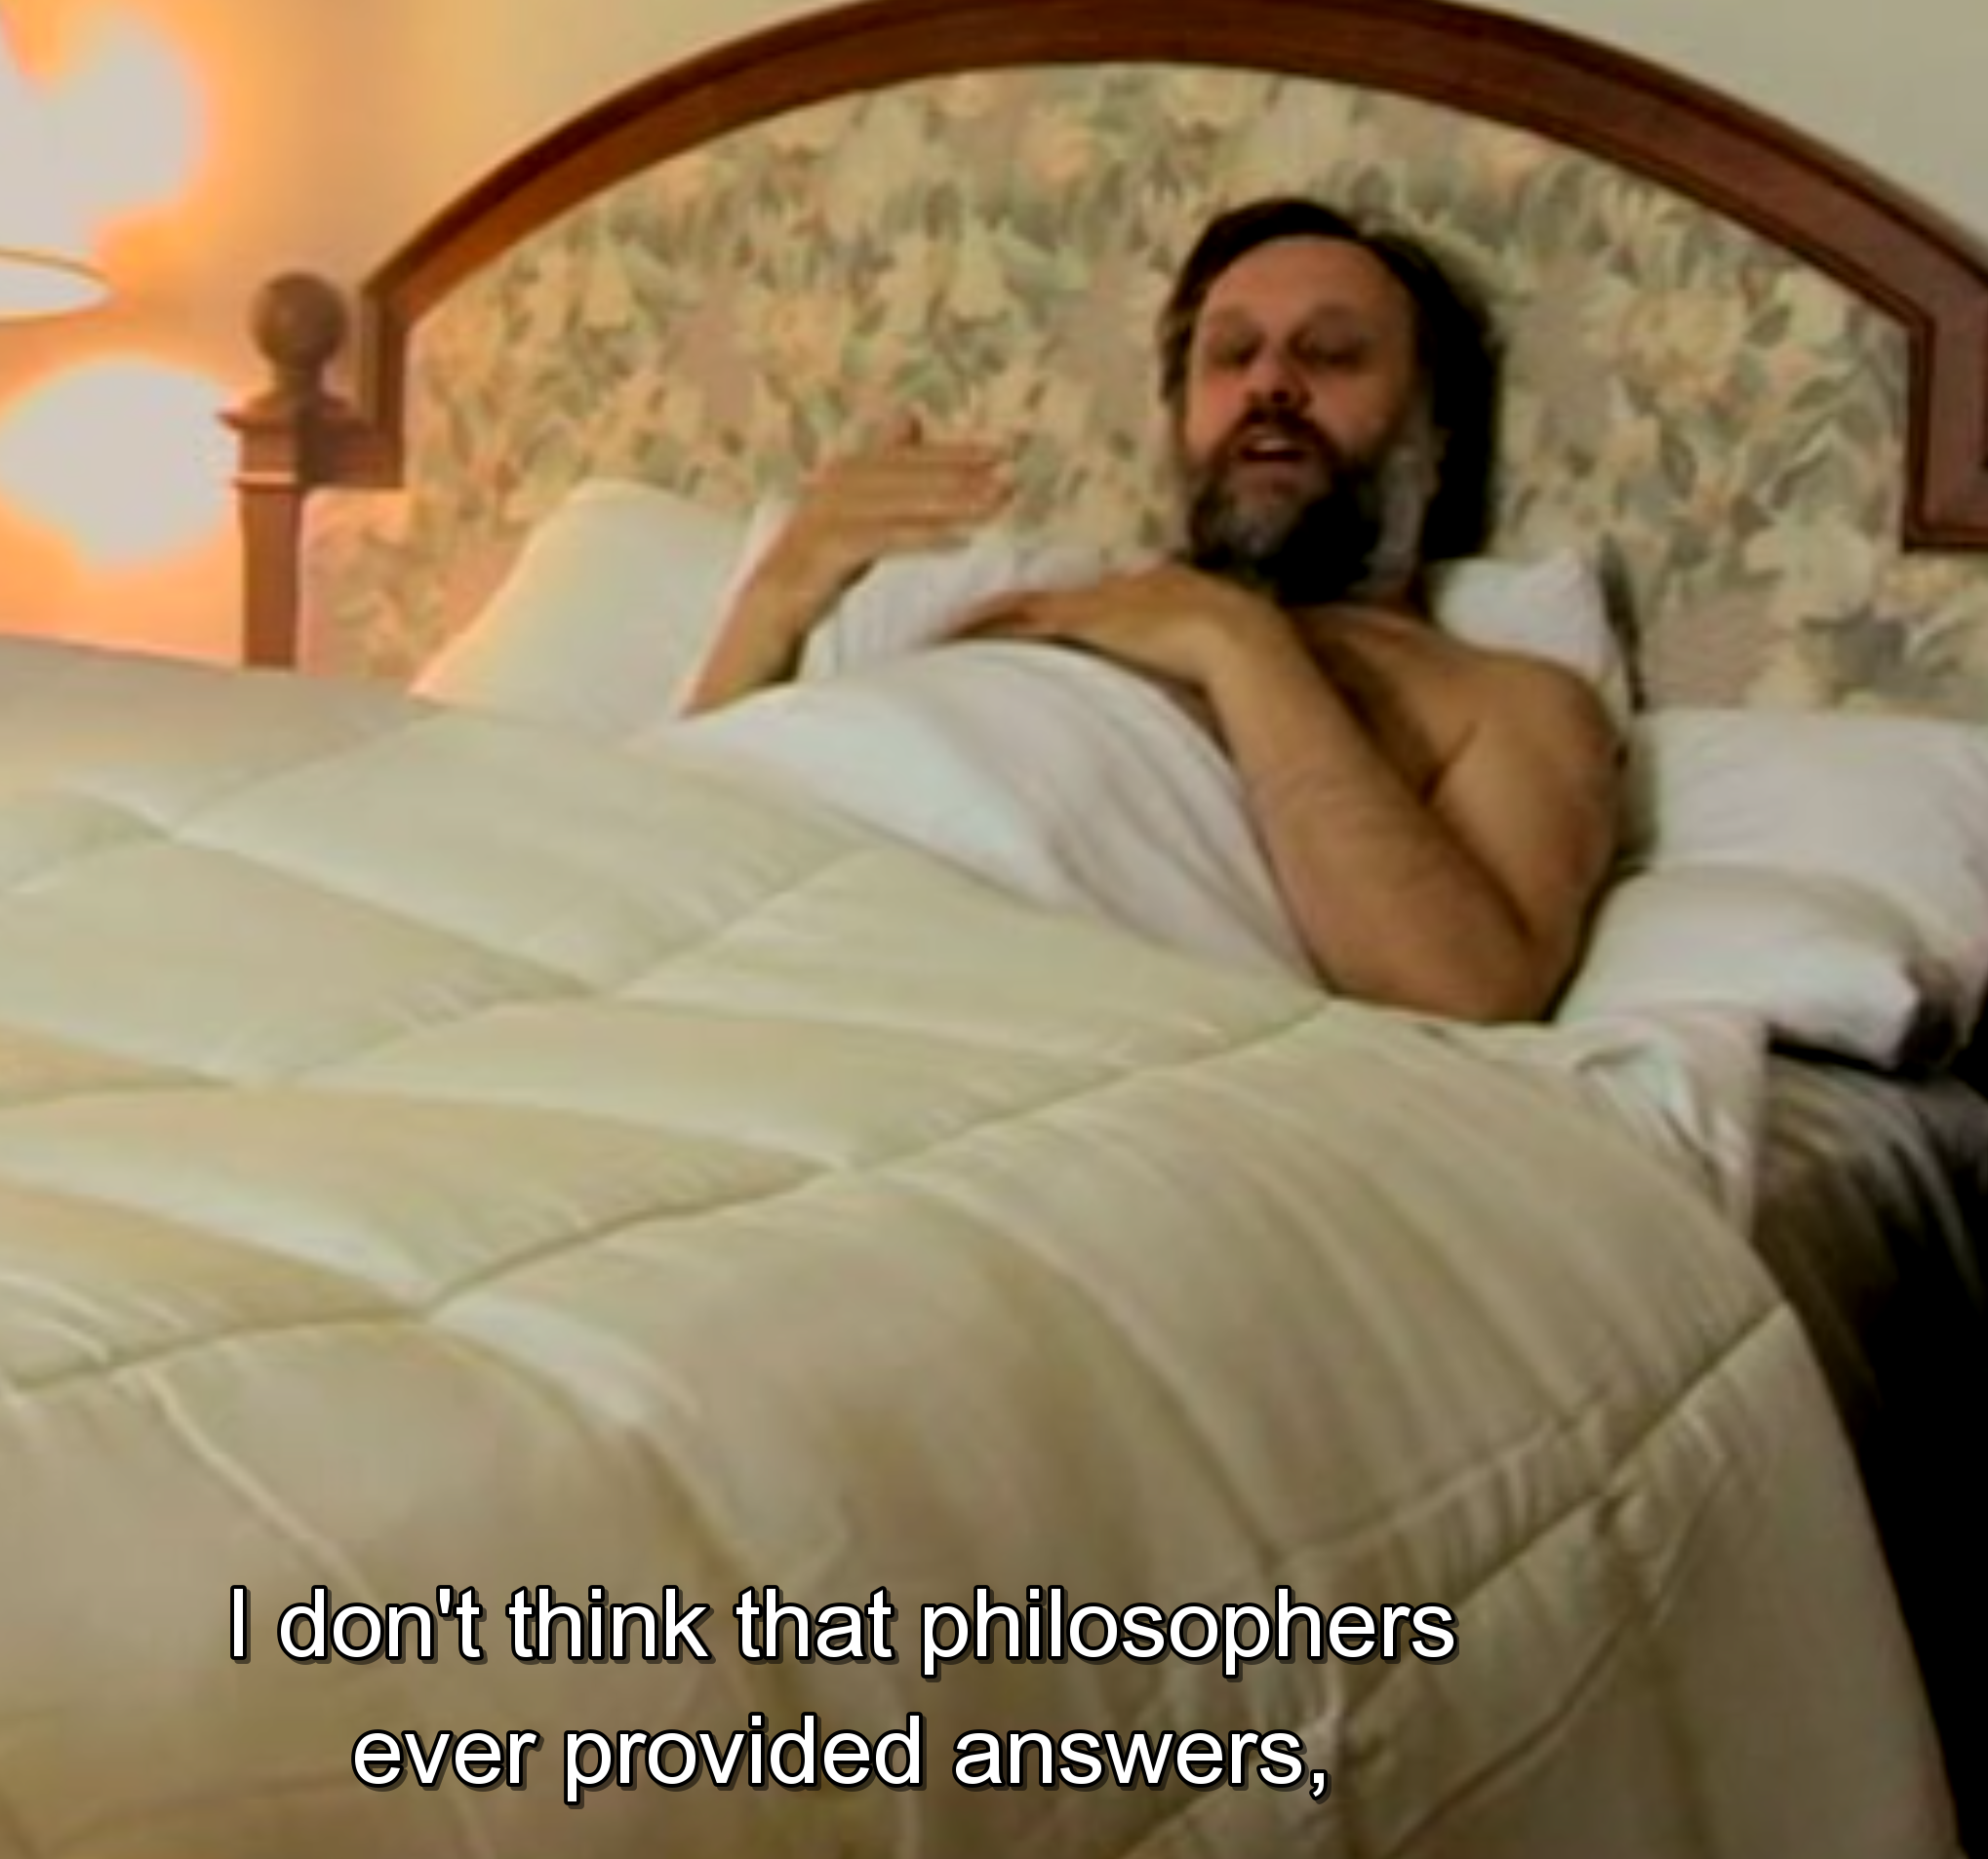
\includegraphics[width=0.5\textwidth]{images/template.png}
%	\caption{Template Bild}
%	\label{fig:template}
%\end{figure}


\end{document}
